\documentclass[hyperref={pdfstartview=Fit}]{beamer}
%\documentclass[hyperref={pdfstartview=Fit,pdfpagemode=FullScreen}]{beamer}
\mode<presentation>
{
  \usetheme{Warsaw}
  \setbeamercovered{transparent}
}
\usepackage[english]{babel}
\usepackage[utf8]{inputenc}
\usepackage{epstopdf}
\usepackage{lmodern}
\usepackage[T1]{fontenc}

\title[Advection equation and antidiffusion]
{Using antidiffusion to solve the advection equation more accurately}

\subtitle{Case study: Smolarkiewicz' iterative approach}

\author[Burger, Wolterink]
{Gerhard Burger \and Jelmer Wolterink}

\institute[Utrecht University]
{
  Scientific Computing\\
  Department of Mathematics\\
  Utrecht University
}

\date[31-Oct-2011] %
{Project presentations SOAC, 31 October 2011}

\subject{Advection equation and antidiffusion}

 \pgfdeclareimage[height=0.5cm]{university-logo}{UU_logo_fullcolor_uncoated_sol_left}
 \logo{\pgfuseimage{university-logo}}



% Delete this, if you do not want the table of contents to pop up at
% the beginning of each subsection:
% \AtBeginSubsection[]
% {
%   \begin{frame}<beamer>{Outline}
%     \tableofcontents[currentsection,currentsubsection]
%   \end{frame}
% }


% If you wish to uncover everything in a step-wise fashion, uncomment
% the following command:

%\beamerdefaultoverlayspecification{<+->}
\newcommand{\imsize}{}

\begin{document}

\begin{frame}
  \titlepage
\end{frame}

\begin{frame}{Outline}
  \tableofcontents
  % You might wish to add the option [pausesections]
\end{frame}

\section{The advection equation in climate modelling}
\subsection{Importance}

\begin{frame}

\begin{block}{Advection}
Transport mechanism of a \textbf{substance} by a \textit{fluid}, due to the fluids \underline{motion} in a particular direction.
\end{block}

Examples in ocean, atmosphere and climate modelling

\begin{itemize}
   \item Transport of \textbf{trace gasses} by \textit{air} due to \underline{wind}
   \item Transport of \textbf{heat} by \textit{ocean water} due to \underline{currents}
   \item Transport of \textbf{warm and moist air} over a colder surface by \textit{air} due to \underline{wind}: advection fog
\end{itemize}

\begin{figure}
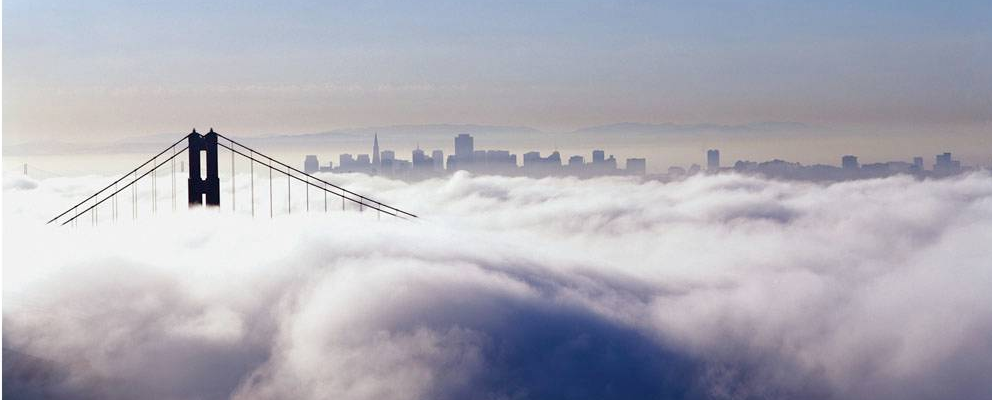
\includegraphics[width=7cm]{advfog.png}
\end{figure}

\end{frame}

\begin{frame}
\frametitle{Advection simulation}

Constraints on advection simulation \cite{rasch}

\begin{itemize}
\item Solutions should contain no unphysical overshoot or undershoot: positive definite
\item Methods should be volume preserving. No loss of matter
\item The solutions should be local: the solution at any one point should not be influenced by what is going on far away from that point
\item The numerical solution should not introduce new extrema in the solution, because the continuous form of the solution would not
\item The method should be cost effective: memory and computational requirements should be sufficiently small so that practical problems may be solved
\end{itemize}

\end{frame}

\subsection{Diffusion}
\frametitle{Problem: diffusion}

When simulating an advective process, we need to discretize space. When doing so, we introduce numerical constraints on the calculation and we get diffusion.

\begin{frame}{Example of diffusion with an upstream scheme}
\renewcommand{\imsize}{0.5\textwidth}
\begin{figure}
\includegraphics<1>[width=\imsize]{animation/anime0.eps}
\includegraphics<2>[width=\imsize]{animation/anime1.eps}
\includegraphics<3>[width=\imsize]{animation/anime2}
\includegraphics<4>[width=\imsize]{animation/anime3}
\includegraphics<5>[width=\imsize]{animation/anime4}
\includegraphics<6>[width=\imsize]{animation/anime5}
\includegraphics<7>[width=\imsize]{animation/anime6}
\includegraphics<8>[width=\imsize]{animation/anime7}
\end{figure}
\end{frame}

\subsection{Antidiffusion methods}

\begin{frame}{Antidiffusion methods 1}
\begin{itemize}
\item Flux-corrected transport (FCT) method (Boris and Book, 1973),
\item self-adjusting hybrid scheme (SAHS) (Harten en Zwas, 1972),
\end{itemize}
   both can be very accurate but require excessive computing time, better is the
\begin{itemize}
   \item hybrid-type scheme based on a Crowley advection scheme (Clark and Hall, 1979),
\end{itemize}
   with more diffusion but half the computation time.
\end{frame}

\begin{frame}{Antidiffusion methods 2}
\begin{itemize}
\item Smolarkiewicz' iterative correction
\end{itemize}
   less time consuming while results are comparable to those of the more complex hybrid schemes
\end{frame}

\section{Case study: Smolarkiewicz}
\subsection{the scheme and method of lines}
\subsection{implementation}
\subsection{numerical results}

\begin{frame}
\frametitle{The scheme}
We start with the following upstream advection equation on staggered grid:
\begin{equation*}
 \psi_i^{N+1} = \psi_i^N - \Big( F \left( \psi_i^N,\psi_{i+1}^N,u_{i+1/2}^N\right)
-F \left( \psi_{i-1}^N,\psi_{i}^N,u_{i-1/2}^N\right) \Big),
\end{equation*}
where
\begin{multline*}
F \left( \psi_i^N,\psi_{i+1}^N,u_{i+1/2}^N\right) =\\
\Big( \left( u_{i+1/2}^N + \abs{u_{i+1/2}^N} \right) \psi_i^N
+ \left( u_{i+1/2}^N - \abs{u_{i+1/2}^N} \right) \psi_{i+1}^N \Big)
\frac{\Delta t}{2 \Delta x}.
\end{multline*}
\end{frame}

\begin{frame}{Writing it out}
Inserting this and collecting terms gives us
\begin{equation*}
\begin{split}
\psi_i^{N+1} &=
\frac{\Delta t}{2 \Delta x} \left( u_{i-1/2}^N + \abs{u_{i-1/2}^N} \right) \psi_{i-1}^N\\
&+ \left(1 - \frac{\Delta t}{2 \Delta x} \left( u_{i+1/2}^N + \abs{u_{i+1/2}^N} - u_{i-1/2}^N + \abs{u_{i-1/2}^N} \right) \right) \psi_i^N\\
&-\frac{\Delta t}{2 \Delta x} \left( u_{i+1/2}^N - \abs{u_{i+1/2}^N} \right) \psi_{i+1}^N\\
\end{split}
\end{equation*}
\end{frame}

\begin{frame}{Writing it out}
We can write this as
\begin{equation*}
\psi_i^{N+1} = \alpha_i \psi_{i-1}^N + \beta_i \psi_i^N +\gamma_i \psi_{i+1}^N, \quad \text{for } i=1,\ldots,M-1,
\end{equation*}
 where we have that
\begin{align*}
\alpha_i &= \frac{\Delta t}{2 \Delta x} \left( u_{i-1/2}^N + \abs{u_{i-1/2}^N} \right),\\
 \beta_i &= \left(1 - \frac{\Delta t}{2 \Delta x} \left( u_{i+1/2}^N + \abs{u_{i+1/2}^N} - u_{i-1/2}^N + \abs{u_{i-1/2}^N} \right) \right),\\
\gamma_i &= -\frac{\Delta t}{2 \Delta x} \left( u_{i+1/2}^N - \abs{u_{i+1/2}^N} \right).
\end{align*}
\end{frame}


\begin{frame}{Matrix form}
We can also write this in matrix form \only<2>\alert{using periodic boundary conditions}
\only<1>{\begin{equation*}
\begin{bmatrix}\psi_{1}^{N+1}\\\psi_{2}^{N+1}\\ \vdots \\\psi_{M-2}^{N+1}\\\psi_{M-1}^{N+1}\end{bmatrix} =
\begin{bmatrix}\beta_1&\gamma_1&&&0\\ \alpha_2&\beta_2&\gamma_2\\ &\ddots&\ddots&\ddots\\&&\alpha_{M-2}&\beta_{M-2}&\gamma_{M-2}\\0&&&\alpha_{M-1}&\beta_{M-1}\\ \end{bmatrix}
\begin{bmatrix}\psi_{1}^N\\\psi_{2}^N\\ \vdots \\\psi_{M-2}^N\\\psi_{M-1}^N\end{bmatrix}
\end{equation*}}
\only<2>{\begin{equation*}
\begin{bmatrix}\psi_{1}^{N+1}\\\psi_{2}^{N+1}\\ \vdots \\\psi_{M-2}^{N+1}\\\psi_{M-1}^{N+1}\end{bmatrix} =
\begin{bmatrix}\beta_1&\gamma_1&&&\alpha_1\\ \alpha_2&\beta_2&\gamma_2\\ &\ddots&\ddots&\ddots\\&&\alpha_{M-2}&\beta_{M-2}&\gamma_{M-2}\\\gamma_{M-1}&&&\alpha_{M-1}&\beta_{M-1}\\ \end{bmatrix}
\begin{bmatrix}\psi_{1}^N\\\psi_{2}^N\\ \vdots \\\psi_{M-2}^N\\\psi_{M-1}^N\end{bmatrix}
\end{equation*}}
\end{frame}
%
% % All of the following is optional and typically not needed.
% \appendix
% \section<presentation>*{\appendixname}
% \subsection<presentation>*{For Further Reading}
%
% \begin{frame}[allowframebreaks]
%   \frametitle<presentation>{For Further Reading}
%
%   \begin{thebibliography}{10}
%
%   \beamertemplatebookbibitems
%   % Start with overview books.
%
%   \bibitem{Author1990}
%     A.~Author.
%     \newblock {\em Handbook of Everything}.
%     \newblock Some Press, 1990.
%
%
%   \beamertemplatearticlebibitems
%   % Followed by interesting articles. Keep the list short.
%
%   \bibitem{Someone2000}
%     S.~Someone.
%     \newblock On this and that.
%     \newblock {\em Journal of This and That}, 2(1):50--100,
%     2000.
%   \end{thebibliography}
% \end{frame}

\bibliographystyle{alpha}
\bibliography{presentation.bib}

\end{document}


